\chapter{xHeinz: a cross-species module discovery tool}
\label{chap:xheinz}

\section{Assigning weights}
\label{sec:weights}

	\subsection{Peptides mappings}

	\subsection{Gene weight through expression profiles}

\section{Algorithmic problem: the \mwccs{} problem}
\label{sec:mip}

	\subsection{Mathematical model}

		We consider the conserved active modules problem in the context of two species networks, which we denote by $G_1 = (V_1, E_1)$ and $G_2 = (V_2, E_2)$.
		Nodes in these networks are labeled by their activity---defined by $w \in \mathbb{R}^{V_1 \cup V_2}$ and conserved node pairs are given by the symmetric relation $R \subseteq V_1 \times V_2$. The aim is to identify two maximal-scoring connected subnetworks, one in each network, such that a given fraction $\alpha$ of module nodes are conserved.
		The formal problem statement is as follows:

		\begin{problem}[Conserved active modules]
  	  	  Given $G_1=(V_1,E_1)$, $G_2 = (V_2,E_2)$, $w \in \mathbb{R}^{V_1 \cup V_2}$ and $R \subseteq V_1 \times V_2$, the task is to find a subset of nodes $V^* = V^*_1 \cup V^*_2$ with 
		$V^*_1 \subseteq V_1$ and $V^*_2 \subseteq V_2$ such that the following 
		properties hold.
		\begin{itemize}
		\item \textbf{Activity:}
  	  	  Node activity scores are given by $w \in
    	 	 \mathbb{R}^{V_1 \cup V_2}$, where positive scores correspond to
    	 	 significant differential expression. For details see Section~\ref{sub:statistical_analysis_and_node_scoring}.
  	  	  %Note that it is up to the user to normalize the node weights as to prevent a bias in activity score towards one species. 
		We require that the sum $\sum_{v \in V^*} w_v$ is maximal.
		\item \textbf{Conservation:}
  	  	  Conserved node pairs are given by the relation $R
    	 	 \subseteq V_1 \times V_2$. We require that at least a certain fraction $\alpha$ of the nodes in the solution must be
  	  	  conserved, that is, $|U^*| \geq \alpha \cdot |V^*|$ where $U^* := \{u \in V_1^*
  	  	  \mid \exists v \in V_2^*: uv \in R\} \cup \{v \in V_2^*
  	  	  \mid \exists u \in V_1^*: uv \in R\}$.
		\item  \textbf{Modularity:}
  	  	  We require that the induced subgraphs $G_1[V^*_1]$ and $G_2[V^*_2]$ are \emph{connected}.
		\end{itemize}
		\end{problem}

		The model allows a trade-off between conservation and activity. If no conservation is
		enforced ($\alpha = 0$), the solution will correspond to two independent
		maximum-weight connected subgraphs. % thereby achieving maximal overall activity.
		Conversely, if complete conservation is required ($\alpha = 1$), the solution
		can only consist of conserved nodes, which results in lower overall
		activity. The user controls this trade-off by varying the value of the parameter
		$\alpha$ from 0 to 1. The activity score 
		monotonically decreases with increasing
		$\alpha$---see Fig.~\ref{fig:exmpl_tradeoff_alpha}. 

		\begin{figure}[t]
			\centering
			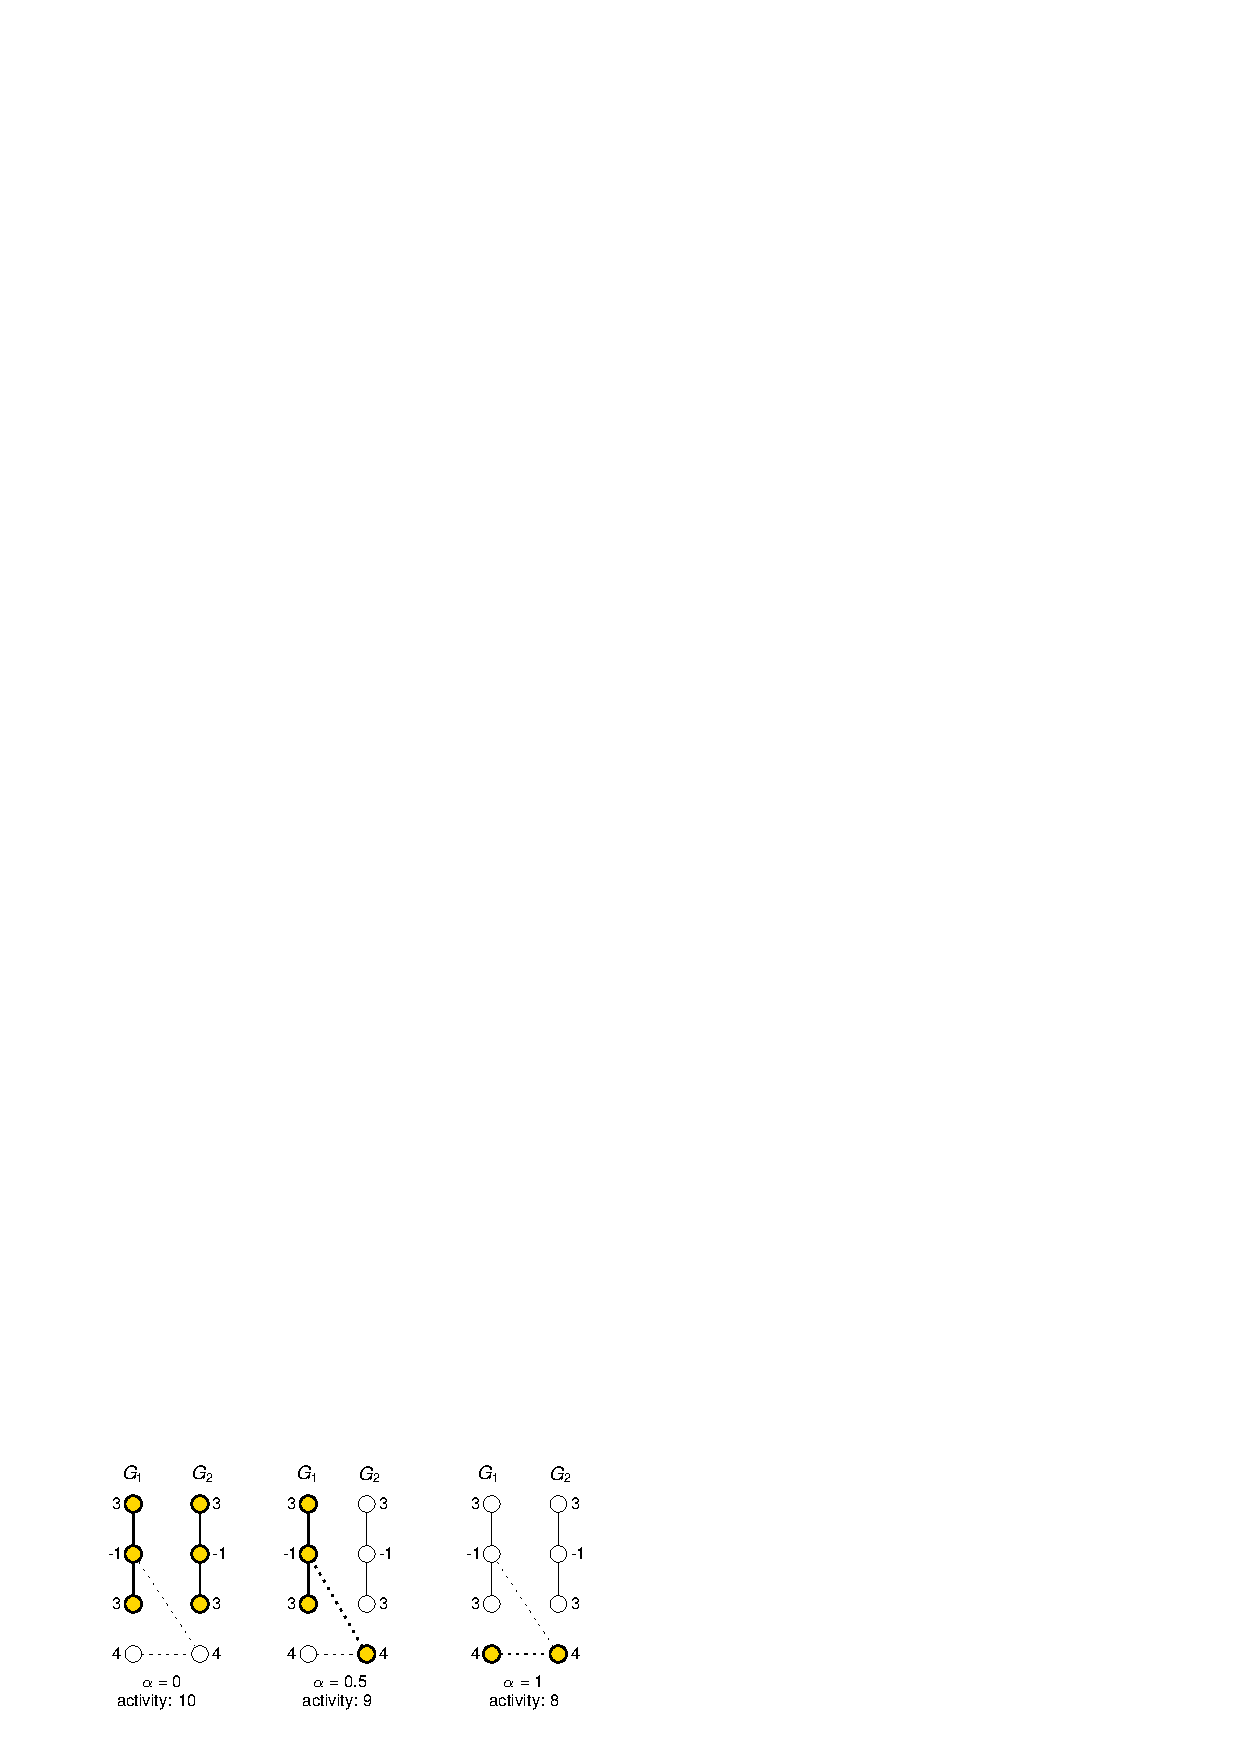
\includegraphics{exmpl_tradeoff_alpha}
			\caption{\textbf{Trade-off between activity and conservation.}
				Three optimal solutions (indicated in yellow) for varying conservation ratios
				$\alpha$ in a toy example instance. Node activities 
				are given next to the
				nodes, conserved node pairs are linked by dotted lines. The activity of a
				conserved module is the sum of the activities of its comprising nodes. The
				parameter $\alpha$ denotes the minimum fraction of nodes in a solution that
				must be conserved, \ie{} connected by a dotted line.}
			\label{fig:exmpl_tradeoff_alpha}
		\end{figure}

		Since the maximum-weight connected subgraph problem, which occurs as a
		subproblem for $\alpha = 0$, is NP-hard \cite{johnson1985np}, the problem of
		finding conserved active modules is NP-hard as well.

	\subsection{Mixed-Integer Linear program}

		We formulate the conserved active modules problem as an integer programming (IP)
		problem in the following way.
		\allowdisplaybreaks
		\begin{alignat}{3}
		\label{eq:obj}  \max\: & \sum_{v \in V_1 \cup V_2} w_v x_v \\
		\label{eq:m_u}  \text{s.t.}\:\: & m_u = \max_{uv \in R} \{ x_u x_v \} & u \in V_1\\
		\label{eq:m_v}            & m_v = \max_{uv \in R} \{ x_u x_v \} & v \in V_2\\
		\label{eq:b}              & \sum_{v \in V_1 \cup V_2} m_v \geq \alpha \sum_{v \in V_1 \cup V_2} x_v &\\
		\label{eq:con}  & \text{$G_1[\mathbf{x}]$ and $G_2[\mathbf{x}]$ are connected}\quad&\\
		\label{eq:vars} & x_v, m_v \in \{0,1\} & v \in V_1 \cup V_2
		\end{alignat}

		Variables $\mathbf{x} \in \{0, 1\}^{V_1 \cup V_2}$
		encode the presence of nodes in the solution, \ie, for all $v \in V_1 \cup
		V_2$ we want $x_v = 1$ if $v \in V^*$ and $x_v = 0$ otherwise. The objective
		function \eqref{eq:obj} uses these variables to express the activity of the
		solution, which we aim to maximize. Variables $\mathbf{m} \in \{0, 1\}^{V_1 \cup V_2}$
		encode the presence of conserved nodes in the solution. Constraints
		\eqref{eq:m_u} encode that a node $u \in V_1$ that is present in the
		solution ($x_u = 1$) is conserved if there exists a related node $v
		\in V_2$ ($uv \in R$) that is also present in the solution ($x_v =
		1$). Similarly, constraints \eqref{eq:m_v} defines conserved nodes in
		$V_2$ that are present in the solution. The fraction of conserved
		nodes in the solution is at least $\alpha$ as captured by
		\eqref{eq:b}. In addition, we satisfy the modularity property by requiring in \eqref{eq:con} that $G_1[\mathbf{x}]$ and $G_2[\mathbf{x}]$ are connected. 

		This formulation satisfies the properties of activity, conservation and modularity.

		\paragraph{Activity.} Variables $\mathbf{x} \in \{0, 1\}^{V_1 \cup V_2}$
		encode the presence of nodes in the solution, \ie, for all $v \in V_1 \cup
		V_2$ we want $x_v = 1$ if $v \in V^*$ and $x_v = 0$ otherwise. The objective
		function \eqref{eq:obj} uses these variables to express the activity of the
		solution, which we aim to maximize.

		\paragraph{Conservation.} Variables $\mathbf{m} \in \{0, 1\}^{V_1 \cup V_2}$
		encode the presence of conserved nodes in the solution. Recall that a
		node $u \in V_1^*$ ($u \in V_2^*$) that is present in the solution is conserved if there
		is another node $v \in V_2^*$ ($v \in V_1^*$) in the solution such that the two
		nodes form a conserved node pair $uv \in R$ ($vu \in R$). This corresponds to
		constraints \eqref{eq:m_u} and \eqref{eq:m_v}. We linearize $x_ux_v$,
		in a standard way, by introducing
		binary variables $\mathbf{z} \in \{0,1\}^R$ such that $z_{uv} =
		x_ux_v$ for all $uv \in R$:
		\allowdisplaybreaks
		\begin{alignat}{3}
		\label{eq:z1} & z_{uv} \leq x_u                 & uv \in R\\
		\label{eq:z2} & z_{uv} \leq x_v                 & uv \in R\\
		\label{eq:z3} & z_{uv} \geq x_u + x_v - 1 \quad & uv \in R\\
		\label{eq:vars2} & z_{uv} \in \{0,1\} & uv \in R
		\end{alignat}
		Subsequently, we model the max function in \eqref{eq:m_u} and \eqref{eq:m_v} as
		follows.
		\allowdisplaybreaks
		\begin{alignat}{3}
		\label{eq:m1}             & m_u \geq z_{uv}                 & uv \in R\\
		\label{eq:m1b}            & m_v \geq z_{uv}                 & uv \in R\\
		\label{eq:m2}             & m_u \leq \sum_{uv \in R}z_{uv}\quad  & u \in V_1\\
		\label{eq:m3}             & m_v \leq \sum_{uv \in R}z_{uv}  & v \in V_2
		\end{alignat}
		We model the required degree of conservation by constraint \eqref{eq:b}.

		\paragraph{Modularity.}
		Constraint \eqref{eq:con} states that the nodes encoded in the solution
		$\mathbf{x}$ induce a connected subgraph in both $G_1$ and $G_2$. There are many ways
		to model connectivity, \eg, using flows or cuts
		\cite{magnanti1995optimal}. Cut-based formulations perform better
		in practice \cite{dilkina2010solving}.
		%The constraints for graph $G_2$ are analogous. 
		Recently, \parencite{alvarez2013maximum} have introduced a cut-based formulation
		that only uses node variables. In an empirical study, the authors show that their formulation
		outperforms other cut-based formulations. We model connectivity along
		the same lines.
		Since the constraints that we will describe are similar for both graphs, we
		introduce them only for graph $G_1 = (V_1, E_1)$. 
		\begin{alignat}{3}
		\label{eq:sumy} & \sum_{v \in V_1} y_v \leq 1 & \\
		\label{eq:y}    & y_v \leq x_v & v \in V_1\\
		\label{eq:cut}  & x_v \leq \sum_{u \in \delta(S)} x_u + \sum_{u \in S} y_u
                  		\quad & v \in V_1, \{v\} \subseteq S \subseteq{V_1}\\
		\label{eq:vars3} & y_v \in \{0,1\} & v \in V_1 \cup V_2
		\end{alignat}
		where $\delta(S) = \{ v \in V_1 \setminus S \mid \exists u \in S: uv
		\in E_1 \}$ denotes the \emph{neighbors} of $S$. The modularity property
		states that $\mathbf{x}$ should induce a connected subgraph in
		$G_1$. We model this by introducing binary variables $\mathbf{y} \in
		\{0, 1\}^{V_1}$ that determine the root node. 
		Constraints \eqref{eq:sumy} and \eqref{eq:y} state that at most
		one node $v \in V_1^*$ is the root node---in which
		case $y_v = 1$. 
		%\comment[guillaume]{Can we give an informal information about the need of
		%having a root node ? An informal overview of the trick that makes it works (not
		%a formal proof) ?} Note that we do not have equality in \eqref{eq:sumy} as it
		%may be the case that $V^*$ is empty or only contains nodes with negative
		%weights\comment[gunnar]{for me the ``Note that...'' sentence can go.}. %% OK,
		%DONE
		Constraints \eqref{eq:cut} state that $x_v$ can only be $1$ if for all sets $S
		\subseteq V$ containing $v$ it holds that either the root node is in $S$ or
		there is a neighbor $u$ of $S$ in the solution. There is an
		exponential number of such constraints. We therefore do not add all
		these constraints to our initial formulation. Instead, we use a
		branch-and-cut approach, that is, at every node of the
		branch-and-bound tree we identify all
		violated constraints and add them to the formulation. Finding violated
		inequalities corresponds to solving a minimum cut problem, which we do using the algorithm
		by \parencite{boykov2004experimental}.

		%In the separation, we also generate back cuts and nested cuts.
		%Details are omitted due to space limitation.

		To further improve the performance, we have strengthened our model with the
		following constraints.
		\begin{alignat}{3}
		\label{eq:y2}   & y_v = 0 & v \in V, w_v < 0\\
		\label{eq:sumy2} & \sum_{u \in V} y_u \geq x_v & v \in V, w_v\geq 0\\
		\label{eq:sym_break} & y_v \leq 1 - x_u \quad & u, v \in V, u < v, w_u \geq 0, w_v \geq 0\\
		\label{eq:1neighbor} & x_v \leq \sum_{u \in \delta(\{v\})} x_u + y_v \quad & v \in V
		\end{alignat}

		As an optimization, we require that the root node must be a non-negatively
		weighted node in \eqref{eq:y2}.
		Constraints \eqref{eq:sumy2} state that if a non-negatively weighted node $v$ is
		present in the solution then there must be a root node. Constraints
		\eqref{eq:sym_break} are symmetry breaking constraints, they require that among
		all non-negatively weighted nodes in the solution, the root node is the smallest
		one---according to some arbitrary order. Finally, constraints
		\eqref{eq:1neighbor} correspond to the cases where the set $S$ in \eqref{eq:cut}
		is a singleton.

\section{Results}
\label{sec:xhres}
